\section{Background}
\subsection{Flash Cache and Disk-head Time (DT)}

The speed of data growth is exponential \cite{turner2014digital}. Storage systems based on a hard disk drive (HDD) eventually fail to meet high-throughput requirements \cite{ren2019hybrid}.
According to \cite{luettgau2018survey}, on average, flash drives deliver 15--20 times the IOPS of hard disk drives and provide throughput 700--1000 times higher. Consequently, a modern storage stack is typically a layered system that serves client I/O requests through a hierarchy of devices. For cost considerations, it is still backed by HDD bulk storage, but to mitigate high I/O demand, a flash cache layer is placed in front to reduce peak backend load. The flash cache stages data in units of fixed-size segments, which allows it to spread out the cost of writing to flash while aligning with HDD read sizes for efficiency.  
The time for one HDD access consists of two parts: seek and move the head, and rotate the platter to read and transfer. The authors define Disk-head Time (DT) Eq.~\eqref{eq:dt-equation} where 
$t_{\text{seek}}$ is the average seek time and $t_{\text{read}}$ is the 
per-byte transfer time \cite{wong2024baleen}. 
\vspace{-0.5em} % adjust as needed
\begin{small}
\begin{equation}
DT_i = t_{\text{seek}} + n \cdot t_{\text{read}}
\label{eq:dt-equation}
\end{equation}
\end{small}

\begin{figure}[t]
    \vspace{-0.8em} % reduce space below
  \centering
  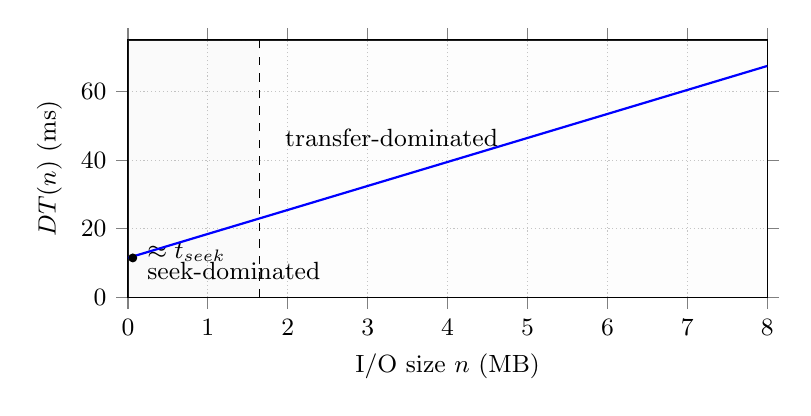
\begin{tikzpicture}
    \begin{axis}[
      width=0.8\columnwidth, height=0.4\columnwidth,
      xmin=0, xmax=8, ymin=0, ymax=75,
      xlabel={I/O size $n$ (MB)}, ylabel={$DT(n)$ (ms)},
      xmajorgrids, ymajorgrids, grid style={densely dotted},
      tick align=outside, tick style={thin},
      label style={font=\small}, tick label style={font=\small}
    ]

      % --- Paper constants (research testbed) ---
      \def\tseek{11.5}      % ms
      \def\bw{143.0}        % MB/s
      \pgfmathsetmacro\slope{1000/\bw}      % ms/MB  ≈ 6.99300699
      \pgfmathsetmacro\nstar{\tseek/\slope} % MB      ≈ 1.6445
      % --- Optional: light regime shading (draw FIRST) ---
      \addplot[draw=none, fill=gray!30, fill opacity=0.12]
        coordinates {(0,0) (\nstar,0) (\nstar,75) (0,75)} -- cycle;
      \addplot[draw=none, fill=gray!10, fill opacity=0.12]
        coordinates {(\nstar,0) (8,0) (8,75) (\nstar,75)} -- cycle;

      % --- Transition boundary ---
      \addplot[dashed] coordinates {(\nstar,0) (\nstar,75)};
      \node[anchor=south east, font=\small, align=right]
        at (axis cs:\nstar,72)
        {$n^\star \approx \pgfmathprintnumber[fixed,precision=2]{\nstar}\,$MB\\
         $t_{\text{seek}} = n^\star \cdot t_{\text{read}}$};
      % --- Labels + seek floor marker ---
      \node[anchor=north west, font=\small] at (axis cs:0.12,13) {seek-dominated};
      \node[anchor=north west, font=\small] at (axis cs:\nstar+0.2,52) {transfer-dominated};
      \addplot[only marks, mark=*, mark size=1.4pt] coordinates {(0.06,\tseek)};
      \node[anchor=west, font=\small] at (axis cs:0.12,\tseek+1.5) {$\approx t_{\text{seek}}$};

      % --- DT line (draw LAST so it’s on top) ---
      \addplot+[no marks, thick, samples=200, domain=0:8] {\tseek + \slope*x};
    \end{axis}
  \end{tikzpicture}
    \caption{DT vs.\ I/O size ($t_{\text{seek}}{=}11.5$\,ms, BW$=143$\,MB/s). 
    The line shows seek- and transfer-dominated regimes; 
    $crossover$ at $n^\star{\approx}1.64$\,MB. 
    Peak DT drives provisioning, which flash caching helps reduce.}
    \vspace{-1em} % reduce space below
  \label{fig:dt-one-line}
\end{figure}

This means HDDs have two constraints upon their throughput: IOPS (input/output operations per second) and sequential transfer bandwidth. Small I/Os are limited by IOPS, and large I/Os will hit the bottleneck of disk bandwidth. 

The authors emphasize DT ``balances IOPS and bandwidth'' and ``generalizes across variable-size I/Os'' \cite{wong2024baleen}. Regardless of request size, using DT as the unified optimization objective allows cache admission and prefetching policies to effectively reduce peak backend load on HDDs. ({Word count:} 252)

\subsection{Episode Model and OPT (Oracle)}
The episodes model groups related cache accesses together instead of tracking every single one individually, which makes flash caching analysis way more manageable. An episode is basically a bunch of accesses to the same data block that would all be hits if we decide to cache that block initially. The first access is always going to be a miss since the data isn't there yet, but everything else would be hits that can be efficiently served from the cache without additional disk activity.

They figure out episode boundaries using LRU eviction age. If two accesses happen within that time window, they are considered part of the same episode. If the gap is longer than eviction age, that’s where one episode ends and maybe a new one starts. This approach has nice advantages. Each episode can be analyzed independently, which makes the math way simpler. It also captures the main trade-off: you pay write cost upfront when caching data, then get benefits from hits during that episode, essentially trading flash endurance for reduced disk load.

The OPT policy uses this to approximate optimal decisions. It generates episodes using assumed eviction age, scores each episode by Disk-head Time saved per storage cost, then picks highest-scoring ones until the write budget runs out. Scoring formula:
\begin{equation}
\small
\label{eq:episode-score}
Score(\text{Episode}) = \frac{DT_{\text{Saved}}(\text{Episode})}{Size(\text{Episode})}
\end{equation}

What’s interesting is how it changes ML training. Instead of learning from individual accesses with complicated dependencies, models focus on episode-level decisions which is much simpler. The episode boundaries represent key decision points where you choose whether to admit something or not, and this abstraction makes model design far more tractable in practice. ({Word count:} 250)

\subsection{ML-Guided Admission (OPT Imitation for Peak DT)}
Machine learning--guided admission in flash caches refers to the use of a predictive model to decide whether a missed block should be inserted into cache under a constrained flash write budget. The approach is based on imitating an offline reference policy, OPT, which provides a near-optimal bound for maximizing disk-head time (DT) savings.

The training of this policy relies on the episode model, which groups all accesses to a block that would be hits if the block were admitted at the first access. Each episode is assigned a cost (number of flash segments written) and a benefit (total DT saved). Episodes are scored by their benefit-to-cost ratio as in Eq.~\eqref{eq:episode-score}.

Episodes are ranked by this score, and the highest scores are selected until the flash write budget is met. These selected episodes provide the labels used to train the admission model. The model is implemented as a binary classifier, typically using gradient boosting machines (GBMs). Input features include metadata describing the request context (namespace, user, block type) and dynamic features capturing recent access frequency. Samples from the first few accesses of each episode are included to capture early decision signals. The classifier outputs an admission probability, and a threshold is calibrated in simulation to achieve the desired flash write rate. The optimization target is Peak Disk-head Time, which reflects the highest backend load over a given interval. By focusing on DT rather than cache hit rate, the admission policy ensures that cache decisions reduce seek and transfer time, aligning with the objective of minimizing backend resource utilization.({Word count:}258)
\begin{figure}[h]
    \centering
    \includegraphics[width=0.85\linewidth]{episode-timeline.pdf} 
    \Description{Timeline of the episode model for a single block: showing cache-resident intervals (green), non-resident intervals, admissions (green arrows), evictions (red arrows), eviction age, and hits (black squares) annotated.}
    \caption{\textbf{Episode Model Timeline.} Two episodes of the same block are illustrated. Each episode begins with an \textbf{Admission} (green arrow), during which the block is \textbf{Cache-Resident} (green interval) and subsequent accesses are hits. If no access occurs for longer than the \textbf{Eviction Age}, the block is \textbf{Evicted} (red arrow), starting a \textbf{Non-Resident Interval}.}
    \label{fig:episode-timeline}
    \end{figure}

\subsection{ML-Guided Prefetching (Coordinated with Admission)}
ML-When is a classifier which aims to decide whether prefetching is worth executing for a given episode to achieve net reductions in DT \cite{wong2024baleen}. 
Based on the admission result made by Baleen's admission model, a binary classifier trained on episodes to imitate OPT \cite{wong2024baleen}---ML-Range proposes a contiguous segment range. ML-When then judges this proposal by estimating the marginal DT benefit of prefetching. If the predicted benefit is greater than a threshold (\(\varepsilon \approx 5 \,\text{ms}\), about half a disk seek), the prefetch is carried out; otherwise, it is skipped. By doing this, Baleen proactively caches the high-value segments of the data that are most likely to reduce the peaks in DT.
\begin{figure}[h]
    \vspace{-0.8em} % reduce space above
    \centering
    
\includegraphics[width=0.4\linewidth]{prefetch.drawio.pdf}
    \Description{Runtime workflow of Baleen system showing ML-Range and ML-When interaction for prefetching.}
    \caption{Runtime workflow of Baleen}
    \vspace{-0.6em} % reduce space below
    \label{fig:baleen-workflow}
\end{figure}
According to the paper, Baleen takes blocks (8 MB) as the data boundary. Within each block, the unit of data is a segment (128 KB). When an episode is admitted, ML-When evaluates ML-Range’s predicted segment range. If ML-When affirms the decision, those segments are prefetched and written into flash cache.
\begin{figure}[t]
    \vspace{-0.8em} % reduce space below
    \centering
    
\includegraphics[width=0.45\linewidth]{training-loop.drawio.pdf}
    \Description{Training loop for Baleen’s admission and prefetching models. 
    Runtime traces are labeled by OPT, then ML-Range and ML-When are trained to 
    approximate these labels for deployment.}
    \caption{Training loop for Baleen. Runtime traces are labeled with OPT; 
    ML-Range and ML-When are trained and deployed, producing new traces 
    to continue the cycle.}
    \vspace{-0.8em} % reduce space below
    \label{fig:training-loop}
\end{figure}

ML-When evaluates ML-Range’s proposals using the benefit formulas
(Eq. 3a–3e in \cite{wong2024baleen}), which quantify the DT saved by prefetching
versus not prefetching. If the predicted benefit exceeds a small threshold
($\varepsilon \approx 5$ ms, about half a disk seek), ML-When approves the
prefetch; otherwise, it is skipped. In this way, only high-value prefetches
are admitted, avoiding unnecessary flash writes.
({Word count:} 253)

\subsection{Baleen-TCO (Cost-Aware Flash Write-Rate Control)}

Total cost of ownership in Baleen was introduced as a consideration in cost controller mainly focused on balancing HDD cost and SSD endurance – more data request and transactions will occur on HDD directly if too little is written in SSD, raising cost due to affected performance costed by high peak DT and the demands for more HDD to maintain performance. Meanwhile, too much data written in the flash cache will accelerate abrasion on the SSD, which also increases cost.
\begin{figure}[H]
    \vspace{-0.8em} % reduce space above
    \centering
    
\includegraphics[width=0.7\columnwidth]{diagram.drawio.pdf} 
    \caption{Control Diagram}
    \Description{A control diagram with labeled inputs (TCO components, DT metrics) and outputs (target write rate).}
    \vspace{-1em} % reduce space below
    \label{fig:diagram}
\end{figure}
In this article, to address this issue, Baleen continuously monitors DT metrics (such as average DT and peak DT) as well as flash memory health metrics (such as remaining write cycles). Flash write rate was calculated dynamically to optimize the cache effect without overuse consumption of flash memory. Baleen achieved a trade-off that minimizing the TCO by protecting flash cache from excessiveness while reducing DT to decrease hard disk load, instead of simply maximizing cache hits. 

Admission policies must also consider flash write amplification and device endurance. For instance, CacheSack optimizes flash cache admission by trading off disk reads and flash writes in Google datacenters \cite{yang2022cachesack}. Recent studies show that sustainable cache designs need to manage backend load and also keep flash write amplification low to extend device life. For instance, WREN\cite{amvrosiadis2024wren} shows how new flash interfaces can help reduce write loads without losing speed. This is similar to Baleen-TCO’s approach because both keep device costs in mind. ({Word count:}240)

\subsection{Writing \& Citation Checklist}

The Background Section is written in cohesive prose, and each section (1.1–1.5) is connected well and makes sense to the next one.

In terms of citation, the background part has the main reference Baleen FAST ’24 paper and four more papers related to flash caching and machine learning–guided caching. The citations include the storage system architectures, data growth and storage problem, and coordinated flash cache management. 

All citations are written in ACM style and no preprints are included. In terms of figures, all required figures are vector diagrams and each figure is accompanied by a descriptive caption. In conclusion, this checklist makes sure the writing, citation, and formatting requirements in the guidelines. ({Word count:}114)

